\chapter{EM-CCD camera calibration}
\section{Andor Basic code listing for automatic image acquisition}
\label{sec:basic-acquisition}
\definecolor{light-gray}{gray}{0.95}

\lstdefinestyle{myframe}{
  basicstyle=\LSTfont,
  % basicstyle=\footnotesize\ttfamily,
  rulesepcolor=\color{gray} ,
  rulecolor = \color{black},
  frame = single,
  % framerule = 0pt,
  backgroundcolor =\color{light-gray}, 
  fontadjust=true,
  breaklines = true,
  showstringspaces=false,
  commentstyle=\itshape,
}
\lstdefinestyle{mymaxima}{
  language=C,
  style=myframe
}
\lstdefinestyle{myclang}{
  language=C,
  style=myframe
}
\lstdefinestyle{myfortran}{
  language=Fortran,
  style=myframe
}
\lstdefinestyle{mymatlab}{
  language=Matlab,
  style=myframe
}
\lstdefinestyle{mylisp}{
  language=Lisp,
  style=myframe
}
\lstdefinestyle{mybasic}{
  language=[Visual]Basic,
  style=myframe
}
\lstdefinestyle{mypython}{
  language=Python,
  showstringspaces=false,
  tabsize=4,
  basicstyle=\ttfamily,
  morekeywords={models, lambda, forms},
  frame = single,
  breaklines = true,
  style=myframe
}


\begin{lstlisting}[style=mybasic]
' This is code for the Basic interpreter in Andor Solis
function ~GetSaturatingExposure()
        SetKineticNumber(1)
        exp=.01
        SetExposureTime(exp)
        run()
        m=maximum(#0,1,512)
        GetSaturatingExposure=exp*10000/(m-100)
        CloseWindow(#0)
return
name$ = "C:\Users\work\Desktop\martin\20111111\scan-em3\ixon_"
print("start")

SetOutputAmp(1)
print("conv_start")
exp= ~GetSaturatingExposure()
print(exp)
SetExposureTime(exp)
SetKineticNumber(20)
SetShutter(0,1)
run()
save(#0,name$ + "conv1_dark.sif")
ExportTiff(#0, name$ + "conv1_dark.tif", 1, 1, 0, 0)
CloseWindow(#0)
CloseWindow(#1)
        
SetShutter(1,1)
run()
save(#0,name$ + "conv1_bright.sif")
ExportTiff(#0, name$ + "conv1 _bright.tif", 1, 1, 0, 0)
CloseWindow(#0)
CloseWindow(#1)

SetOutputAmp(0)
SetShutter(1,1)
for i = 40 to 300 step 10
        SetGain(i)
        exp=~GetSaturatingExposure()
        print(exp)
        SetExposureTime(exp)
        SetKineticNumber(20)
        SetShutter(0,1)
        run()
        save(#0,name$ + str$(i) + "_dark.sif")
        ExportTiff(#0, name$ + str$(i) + "_dark.tif", 1, 1, 0, 0)
        CloseWindow(#0)
        CloseWindow(#1)
        SetShutter(1,1)
        run()
        save(#0,name$ + str$(i) + "_bright.sif")
        ExportTiff(#0, name$ + str$(i) + "_bright.tif", 1, 1, 0, 0)
        CloseWindow(#0)
        CloseWindow(#1)
next

SetOutputAmp(1)
print("conv_end")
exp= ~GetSaturatingExposure()
print(exp)
SetExposureTime(exp)
SetKineticNumber(20)
SetShutter(0,1)
run()
save(#0,name$ + "conv2_dark.sif")
ExportTiff(#0, name$ + "conv2_dark.tif", 1, 1, 0, 0)
CloseWindow(#0)
CloseWindow(#1)
        
SetShutter(1,1)
run()
save(#0,name$ + "conv2_bright.sif")
ExportTiff(#0, name$ + "conv2 _bright.tif", 1, 1, 0, 0)
CloseWindow(#0)
CloseWindow(#1)
\end{lstlisting}

\begin{table}[!htbp]
  \centering
%  \begin{tabular}{|l|l|l|l|l|l|l|l|}
  \begin{tabular}{r l l r  l r l}
\hline
$\textsf{gain}_\textrm{software}$ & $1/(M\cdot M_\textrm{pre})$ & $N_r$ & $N_{(M)}/(W\times H)$ &  \textsf{exposure} & $N_{(M)}'/(W\times H)$ & $1/F_n$ \\
 & [e/ADU] & [e/px] & [e/px] & [ADU] & [s] & [e/(px s)]  \\
\hline
conv1 & 1.3165 & 7.189 & 3008.66      & 0.2016 & 14923 & 0.981 \\
50 & 0.1160 & 0.486 & 260.05 & 0.0289 & 8995 & 0.591 \\
60 & 0.0984 & 0.406 & 225.46 & 0.0249 & 9054 & 0.595 \\
70 & 0.0841 & 0.349 & 190.52 & 0.0212 & 8983 & 0.591 \\
80 & 0.0729 & 0.305 & 165.24 & 0.0186 & 8907 & 0.586 \\
90 & 0.0680 & 0.288 & 150.54 & 0.0161 & 9368 & 0.616 \\
100 & 0.0611 & 0.262 & 128.47 & 0.0136 & 9427 & 0.620 \\
110 & 0.0550 & 0.241 & 121.11 & 0.0129 & 9409 & 0.619 \\
120 & 0.0510 & 0.228 & 113.71 & 0.0120 & 9498 & 0.624 \\
130 & 0.0465 & 0.211 & 106.66 & 0.0112 & 9541 & 0.627 \\
140 & 0.0433 & 0.201 & 96.95 & 0.0101 & 9564 & 0.629 \\
150 & 0.0405 & 0.192 & 89.68 & 0.0093 & 9671 & 0.636 \\
160 & 0.0380 & 0.183 & 87.24 & 0.0090 & 9656 & 0.635 \\
170 & 0.0359 & 0.175 & 81.56 & 0.0084 & 9739 & 0.640 \\
180 & 0.0339 & 0.169 & 79.80 & 0.0081 & 9863 & 0.648 \\
190 & 0.0321 & 0.163 & 74.00 & 0.0075 & 9806 & 0.645 \\
200 & 0.0305 & 0.158 & 72.57 & 0.0073 & 9878 & 0.649 \\
210 & 0.0292 & 0.155 & 69.44 & 0.0070 & 9944 & 0.654 \\
220 & 0.0280 & 0.150 & 67.69 & 0.0068 & 9971 & 0.656 \\
230 & 0.0268 & 0.147 & 65.63 & 0.0065 & 10057 & 0.661 \\
240 & 0.0257 & 0.188 & 63.90 & 0.0063 & 10131 & 0.666 \\
250 & 0.0244 & 0.140 & 62.52 & 0.0062 & 10026 & 0.659 \\
260 & 0.0237 & 0.137 & 62.86 & 0.0062 & 10078 & 0.663 \\
270 & 0.0229 & 0.135 & 63.17 & 0.0062 & 10130 & 0.666 \\
280 & 0.0221 & 0.133 & 63.64 & 0.0062 & 10204 & 0.671 \\
290 & 0.0214 & 0.130 & 63.38 & 0.0062 & 10162 & 0.668 \\
300 & 0.0205 & 0.128 & 63.20 & 0.0062 & 10133 & 0.666 \\
conv2 & 1.5953 & 8.768 & 8198.86 & 0.5291 & 15496 & 1.019 \\
\hline
\end{tabular}
%  \includegraphics[width=12cm]{../app_cam/ixon3}
\caption{Comparison of read noise for different EM-gain settings
  (first column) of the Andor IXon3. $W$ and $H$ are the size of the sensor (in pixels). The value $N_{(M)}'$
  estimates the number of photoelectrons the detector would have
  seen with \unit[1]{s} integration time and is used to calculate
  the excess noise factor in the last column. In EM-mode the fastest
  readout speed was used \unit[10]{MHz} with vertical shift speed of
  \unit[1.7]{$\mu$s}.}
  \label{tab:ixon-table}
\end{table}

\newpage

\section{Python code listing for the read noise evaluation}
\label{sec:python-readnoise-eval}

\begin{figure}
  \centering
  \pdfinput{17cm}{ixon_conv1}
  \pdfinput{17cm}{ixon_300}
  \caption{Readnoise evaluation using the Python code in section
    \ref{sec:python-readnoise-eval}{\bf top:} Conventional readout of
    an Andor IXon3 camera. {\bf bottom:} readout with an EM-gain
    setting of 300 on the same camera with identical sample. {\bf
      left:} 2D histogram of per pixel variances against binned
    intensities. {\bf middle:} variance of 20 dark images. {\bf
      right:} mean of 20 dark images.}
  \label{fig:ixon}
\end{figure}
  


\begin{lstlisting}[style=mypython]
#!/usr/bin/env python
# ./ti.py /media/backup/andor-ultra-ixon/martin/20111111/scan-em3/ ultra 2700
import sys
import os

import matplotlib
matplotlib.use('Agg')

from pylab import *
from libtiff import TIFFfile, TIFFimage
from scipy import stats

seterr(divide='ignore')

folder = sys.argv[1]
cam = sys.argv[2]
gain = sys.argv[3]

def readpics(gain,cam='ixon_',isdark=False):
    print 'loading ', os.path.join(folder,cam) + '_' + gain + '_bright.tif'
    fg=TIFFfile(os.path.join(folder,cam) + '_' + gain + '_bright.tif')
    bright,bright_names=fg.get_samples()
    bg=TIFFfile(os.path.join(folder,cam) + '_' + gain + '_dark.tif')    
    dark,dark_names=bg.get_samples()
    return (bright[0],dark[0])

(f,b) = readpics(gain=gain,cam=cam)

bg=mean(b,axis=0)
v=var(f,axis=0)
i=mean(f,axis=0)

ny,nx=64,128
H,y,x=histogram2d(v.flatten(),i.flatten(),bins=[ny,nx],
                  range=[[0,v.max()],[0,i.max()]])
extent = [x[0], x[-1], y[0], y[-1]] 
acc=zeros(x.shape,dtype=float64)
accn=zeros(x.shape,dtype=int64)
s=nx/i.max()
for ii,vv in nditer([i,v]):
    p=round(ii*s)
    acc[p]+=vv
    accn[p]+=1   

fig=figure(figsize=(24, 8),dpi=300)
hold(False)
title('bal')
subplot(1,3,1)
imshow(log(H), extent=extent,
           aspect='auto', interpolation='none',origin='lower')
hold(True)
ax=x[nonzero(accn)]
ay=acc/accn
ay=ay[nonzero(accn)]
l=round(.6*len(ax))
bx=ax[0:l]
by=ay[0:l]
plot(ax,ay,'r+')
slope,intercept,rval,pval,stderr=stats.linregress(bx,by)
plot(ax,polyval([slope,intercept],ax))
xlabel('intensity/ADU')
ylabel(r'variance/ADU$^2$')
real_gain=1/slope # unit electrons/ADU
read_noise=sqrt(var(b))*real_gain # electrons RMS per pixel
mean_elecs=(mean(f)-mean(b))*real_gain # photoelectrons electrons per pixel
print gain,cam,real_gain,read_noise,mean_elecs,mean(b),rval,pval,stderr
tit='EM-gain: %s, cam: %s, real gain: %.2f e/ADU\n
read noise: %.2f e RMS/pixel, mean: %.2f e/pixel, offset: %.2f'
% (gain,cam,real_gain,read_noise,mean_elecs,mean(b))
title(tit)
subplot(1,3,2)
imshow(var(b,axis=0))
title('variance of darkimages')
colorbar()
subplot(1,3,3)
imshow(mean(b,axis=0))
title('mean of darkimages')
colorbar()
show()
fig.savefig(cam+'_'+gain+'.png')
\end{lstlisting}


\chapter{Optical sectioning by structured illumination}
\comment{
\jpginput{}{m_phase}{}
}


\begin{figure}[H]
  \centering
  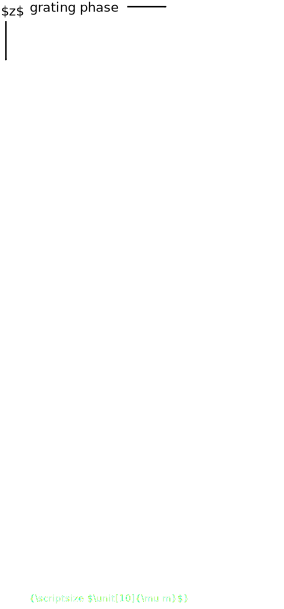
\includegraphics[height=.6\textheight]{m_phase}
  \caption{Structured illumination images of the same of the beads
    from \figref{fig:m_wf}. Of each $z-$slice (rows) four exposures
    with different grating phase (columns) were captured.}
  \label{fig:m_phase}
\end{figure}


\chapter{Mapping between focal plane SLM and camera}
\label{sec:app_map}
\section{Rigid coordinate transformation}
Each term of the sum in equation
\ref{eqn:rigid-sum} on page \pageref{eq:rigid-sum} can be expressed as
two scalar terms:
\begin{align}
  \mathcal{Q}=\sum_i^n&
  \abs{s(\cos\phi r^c_{ix}+q\sin\phi r^c_{iy})+t_x-r^d_{ix}}^2
  +
  \abs{s(-\sin\phi r^c_{ix}+q\cos\phi r^c_{iy})+t_y-r^d_{iy}}^2
\end{align}

The following Maxima code will find the solution to the least squares
problem:
\begin{lstlisting}[style=mymaxima]
load(minpack)$
q:-1;
g(s,p,tx,ty):=[s*( cos(p)*<cx>+q*sin(p)*<cy>)+tx-<dx>,
               s*(-sin(p)*<cx>+q*cos(p)*<cy>)+ty-<dy>, ... ]$
minpack_lsquares(g(s,p,tx,ty), [s,p,tx,ty], [0.88,-3.1,1200,-20]);
\end{lstlisting}
I define the function \verb!g! to contain all the terms of the sum.
This can easily written by a program that constructs the lines
according to the given pattern, replacing \verb!<cx>!, \verb!<cy>!
with camera coordinates and \verb!<dx>!, \verb!<dy>! with display
coordinates.
\comment{$}
The function \verb!minpack_lsquares! calls the subroutine \verb!lmder!
which was originally developed for the Fortran\footnote{Rather than
  calling a Fortran library Maxima calls a version of this function
  that was automatically translated into Common Lisp via {\sf f2cl}.}
package \verb!minpack!.

\begin{lstlisting}[style=myfortran]
c     subroutine lmder (http://www.netlib.org/minpack/lmder.f)
c     the purpose of lmder is to minimize the sum of the squares of
c     m nonlinear functions in n variables by a modification of
c     the levenberg-marquardt algorithm. the user must provide a
c     subroutine which calculates the functions and the jacobian.
c     the subroutine statement is
c       subroutine lmder(fcn,m,n,x,fvec,fjac,ldfjac,ftol,xtol,gtol,
c                        maxfev,diag,mode,factor,nprint,info,nfev,
c                        njev,ipvt,qtf,wa1,wa2,wa3,wa4)
\end{lstlisting}
The reason for using Maxima is, that it calculates the symbolic
Jacobian for the problem. This makes it straight forward to change the
simple rigid transform to a model with more parameters.

The following Common Lisp code shows how the result of the
optimization can be used to initialize the OpenGL modelview matrix to
transform objects in its buffer, so that they will appear at the given
positions on the camera.
 
\begin{lstlisting}[style=mylisp]
(defun load-cam-to-lcos-matrix (&optional (x 0s0) (y 0s0))
  (let* ((s 0.828333873909549) (sx  s)        (sy  (- s))
         (phi -3.102)          (sp (sin phi)) (cp (cos phi))
         (tx 608.433)          (ty 168.918)
         (a (make-array (list 4 4) :element-type 'single-float
             :initial-contents
             (list (list (* sx cp)    (* sy sp)  .0   (+ x tx))
                   (list (* -1 sx sp) (* sy cp)  .0   (+ y ty))
                   (list .0           .0        1.0   .0)
                   (list .0           .0         .0  1.0)))))
    (gl:load-transpose-matrix (sb-ext:array-storage-vector a))))    
\end{lstlisting}  
Alternatively, here is the equivalent code in C (with different
parameters):

\begin{lstlisting}[style=myclang]
float m[4*4]; // OpenGL Modelview Matrix
float s=-.8749328910202312,
      sx=s,sy=-s,phi=-.8052030670943575,
      cp=cos(phi),sp=sin(phi),
      tx=1456.71806436377,
      ty=910.4787738693659;
  m[0]=   sx*cp;   m[4]=sy*sp;   m[8] =0;    m[12]=tx; 
  m[1]=-1*sx*sp;   m[5]=sy*cp;   m[9] =0;    m[13]=ty; 
  m[2]=0;          m[6]=0.;      m[10]=1;    m[14]=0;  
  m[3]=0;          m[7]=0.;      m[11]=0;    m[15]=1;  
glMatrixMode(GL_MODELVIEW);
glLoadMatrixf(m);
\end{lstlisting}
\section{Image processing: Localizing bright spots on the camera}
The following Matlab listing shows how to open the image files:
% cd /mnt/scan 

\begin{lstlisting}[style=mymatlab]
%% load the files
% 0 .. 99 spot images
% only 10..99 usable because the first are on border and not illuminated
  a = newim(1392,1040,103); for i=0:102
  % Andor's FITS format isn't read correctly
  % correct this by adding 2^15
  a(:,:,i) = 2^15 + readim(sprintf('o%03d.fits',i));
  end
\end{lstlisting}
  Of the 103 images, that are loaded into \verb!a!, the first 100
  contain spots and the image at the zero-based index 102 is the
  uniformly illuminated image shown in \figref{fig:rigid-pics} left.
  The other two images at indices 100 and 101 are two centered disks
  with different diameters and are not used here.

  \begin{lstlisting}[style=mymatlab]
    bright = squeeze(a(:,:,102)); % histogram of uniformly illuminated
    % image has minimum at 800 ADU
    mask = gaussf(bright,8) > 800; % create mask with illuminated area
    bg = 510; % the background is be 510 ADU

    posmax = newim(100,2); for i = 10:99
    % correct for sample non-uniformity
    corr = (squeeze(a(:,:,i)) - bg) / bright * mask;
    % find coordinates of maximum
    [coords,vals]=findmaxima(gaussf(corr,32)); [valss,valsind] =
    sort(vals); % sort coordinates by intensity
    tmp = coords(valsind,:); % collect the maximum with highest
    posmax(i,:) = tmp(end,:); % intensity into result
    end
  \end{lstlisting}

  The DIPimage toolbox provides the function \verb!findmaxima!, that
  locates all local maxima in an image with subpixel accurac y. I
  sort the result by gray value and only use the biggest.  The
  measured 100 camera coordinate pairs in \verb!posmax! correspond to
  $\r^c_i$ in equation \ref{eq:rigid-sum}.
 
  From Matlab I create the file \verb!fit.max! with batch commands
  for Maxima. Then I run Maxima. When it is finished after a few
  seconds, the file \verb!max.out! will contain the four fitted
  parameters.
 
\begin{lstlisting}[style=mymatlab]
    c = double(posmax)'; cmd =
    ''; % collect equations in maxima format
    for i=10:99 dx = num2str(400+50*mod(i,10)); dy =
    num2str(500+50*floor(i./10)); cx = num2str(c(i+1,1)); cy =
    num2str(c(i+1,2)); cmd=[cmd ' s*( cos(p)*' cx '+q*sin(p)*' cy
    ')+tx-' dx ', ...  s*(-sin(p)*'cx '+q*cos(p)*' cy ')+ty-' dy ','];
    end cmd(:,end) = []; % delete last comma

% load the fitting package and start defining the merit function g
    pre = 'load(minpack)$ q:-1; g(s,p,tx,ty):=[';
% now put cmd between
% call the fitting function and store the parameters into max.out
    cod = [']$
    fit:minpack_lsquares(g(s,p,x,y),[s,p,x,y],[.88,-1.3,1200,-20]);'
    ...  'write_data(fit[1],"max.out");']

    fid = fopen('fit.max','w'); % write maxima commands into file
    fwrite(fid,[pre cmd cod]); fclose(fid);
    [max_status,max_result]=system('maxima -b
    fit.max'); % execute maxima
  \end{lstlisting}
  We load the transformation parameters back into Matlab and create
  the diagram \figref{fig:rigid-compare} to visualize, how well the
  transform matches camera and display coordinates.

 \begin{lstlisting} [style=mymatlab]
% load rigid transformation parameters from the file into matlab
  params = load('max.out')'; scale = params(1); phi = params(2); tx =
  params(3); ty = params(4);

  mirr = -1; R = [cos(phi),mirr*sin(phi); -sin(phi),mirr*cos(phi)]; T
  = [tx ty]';

  %% plot the two grids on top of each other
  mapped = zeros(100,2); for
  i=11:100 % camera coordinates into display coordinates
  mapped(i,:) = (scale*R*q(i,:)'+T)'; end

  dpos = zeros(100,2); for i=0:99 % calculate display points
  dpos(i+1,1) = 400+50*mod(i,10); dpos(i+1,2) = 500+50*floor(i./10);
  end

  hold off; plot(dpos(:,1),dpos(:,2),'.'); hold on;
  plot(mapped(11:end,1),mapped(11:end,2),'r+');
  % \end{lstlisting}

% print -depsc2 /home/martin/thesis/kielhorn/rigid/rigid-compare
